\begin{figure}
    \centering
    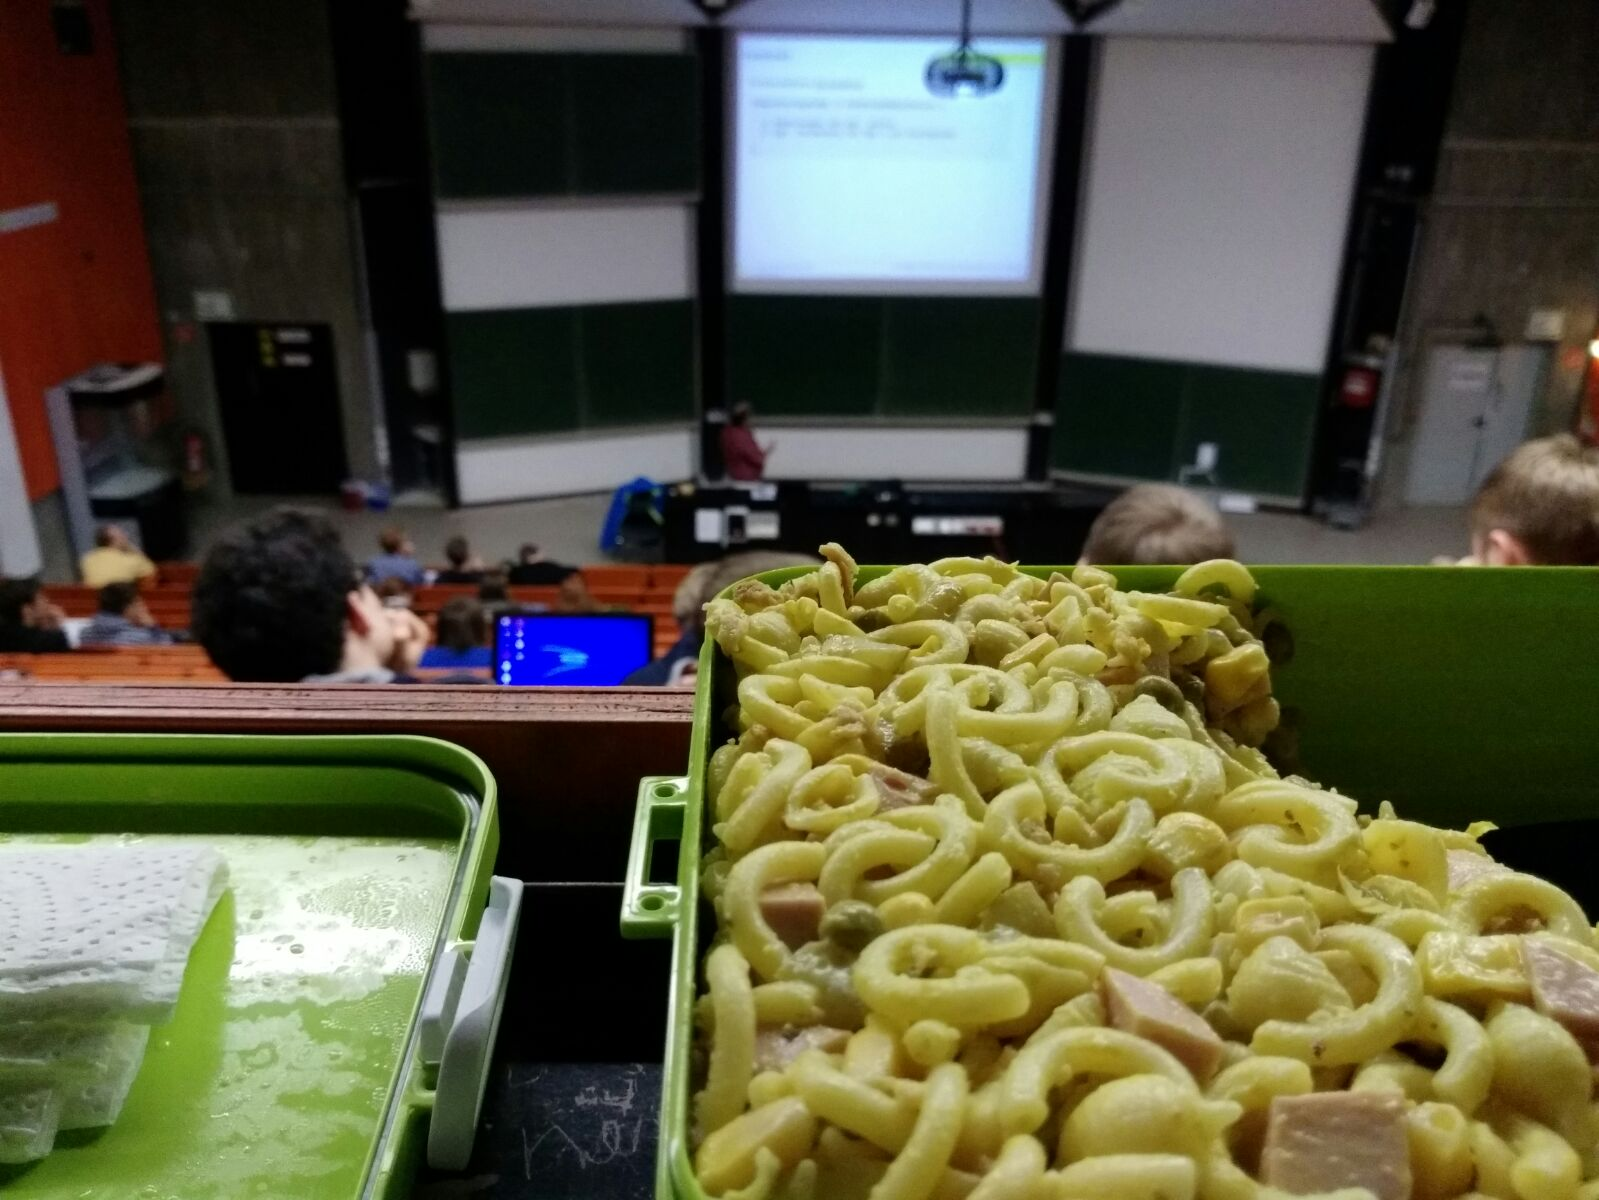
\includegraphics[width=.5\textwidth]{lasse/Nudelsalat.jpeg}
\end{figure}

\begin{recipe}
    [ % Optionale Eingaben
        preparationtime = {\unit[40]{min}},
        portion = \portion{6-10},
        %calory,
        source = Lasse
    ]
    {DER Nudelsalat}
    
    \introduction{
        \# orgasmischlecker
    }
    

    \ingredients
    {% Zutatenliste
        \unit[500]{g} & Suppennudeln \\
        \unit[1]{Dose} & Mais \\
        \unit[1]{Dose} & Erbsen \\
        \unit[1]{Gl} & Gewürzgurken \\
        \unit[1]{}  & Kleine Fleischwurst \\
         & Majo \\
         & Röstzwiebeln \\
        Gewürze & Pfeffer, Salz, Curry
    }
    
    \preparation
    { % Schrittweise Zubereitung
        \\
        Die Nudeln in Salzwasser nach Anleitung al Dente kochen und abkühlen lassen oder mit kaltem Wasser abspülen. \\
        
        Mais und Erbsen abtropfen lassen und die Gurken (gegebenenfalls auch die FLeischwurst) in ähnlich große Stücke schneiden. \\ 
        
        Alles in eine große Schüssel geben und verrühren. Drei bis vier große aufgehäufte Löffel Majonese mit verrühren. Mit Salz und Pfeffer und ORDENTLICH Curry würzen, bis keine Majofarbigen Flecken verbleiben. \\ 
        
        Röstzwiebeln am besten frisch auf dem Teller dazu nehmen. 
        
    }
    
    \hint
        {% Hinweise
        Nudeln können persönlich optimiert werden, ich empfehle 50/50 Eiermuscheln und Gabelspaghetti für die perfekte Löffelkonsistenz. 
        
        Natürlich auch ohne Fleischwurst möglich und vegane Remoulade o.Ä. ersetzen gut die Majo. (Wunderschlag wirkt Wunder). 
        
        Das Bild wurde von einem fleißigen Koch generiert.
        }
    
    \end{recipe}
    